\documentclass[12pt,a4paper]{report}
\usepackage{graphicx}
\usepackage[frenchb]{babel}
\addto\captionsfrench{\renewcommand{\chaptername}{Chapitre}}
\usepackage[utf8]{inputenc}
\usepackage{caption}
\captionsetup[figure]{labelformat=empty}
\begin{document}
\begin{titlepage}


	\centering
	
\includegraphics[width=0.20\textwidth]{ensea.png}\par\vspace{1cm}
	{\scshape\LARGE Ecole Nationale Supérieure de l'Electronique et de ses Applications \par}
	\vspace{1cm}
	{\scshape\Large Projet Latéral Transversal\par}
	\vspace{1.5cm}
	{\huge\bfseries Tales of Kornwal\par}
	\vspace{2cm}
	{\Large\itshape OUAZZAGHTI Reda\par et\par ZOUHDI Zakaria\par}
	\vfill
	Projet de troisième année supervisé par\par
	M.~\textsc{Granier} et Prof.~\textsc{Gosselin}

	\vfill

% Bottom of the page
	{\large 29 Septembre 2016\par \tiny \begin{flushleft}
	Version 1.1 du 29/09/16 \today
\end{flushleft}	 }

\end{titlepage}

\tableofcontents
    \chapter{Objectif}
    \section{Présentation générale}
    \begin{figure*}[htp]
    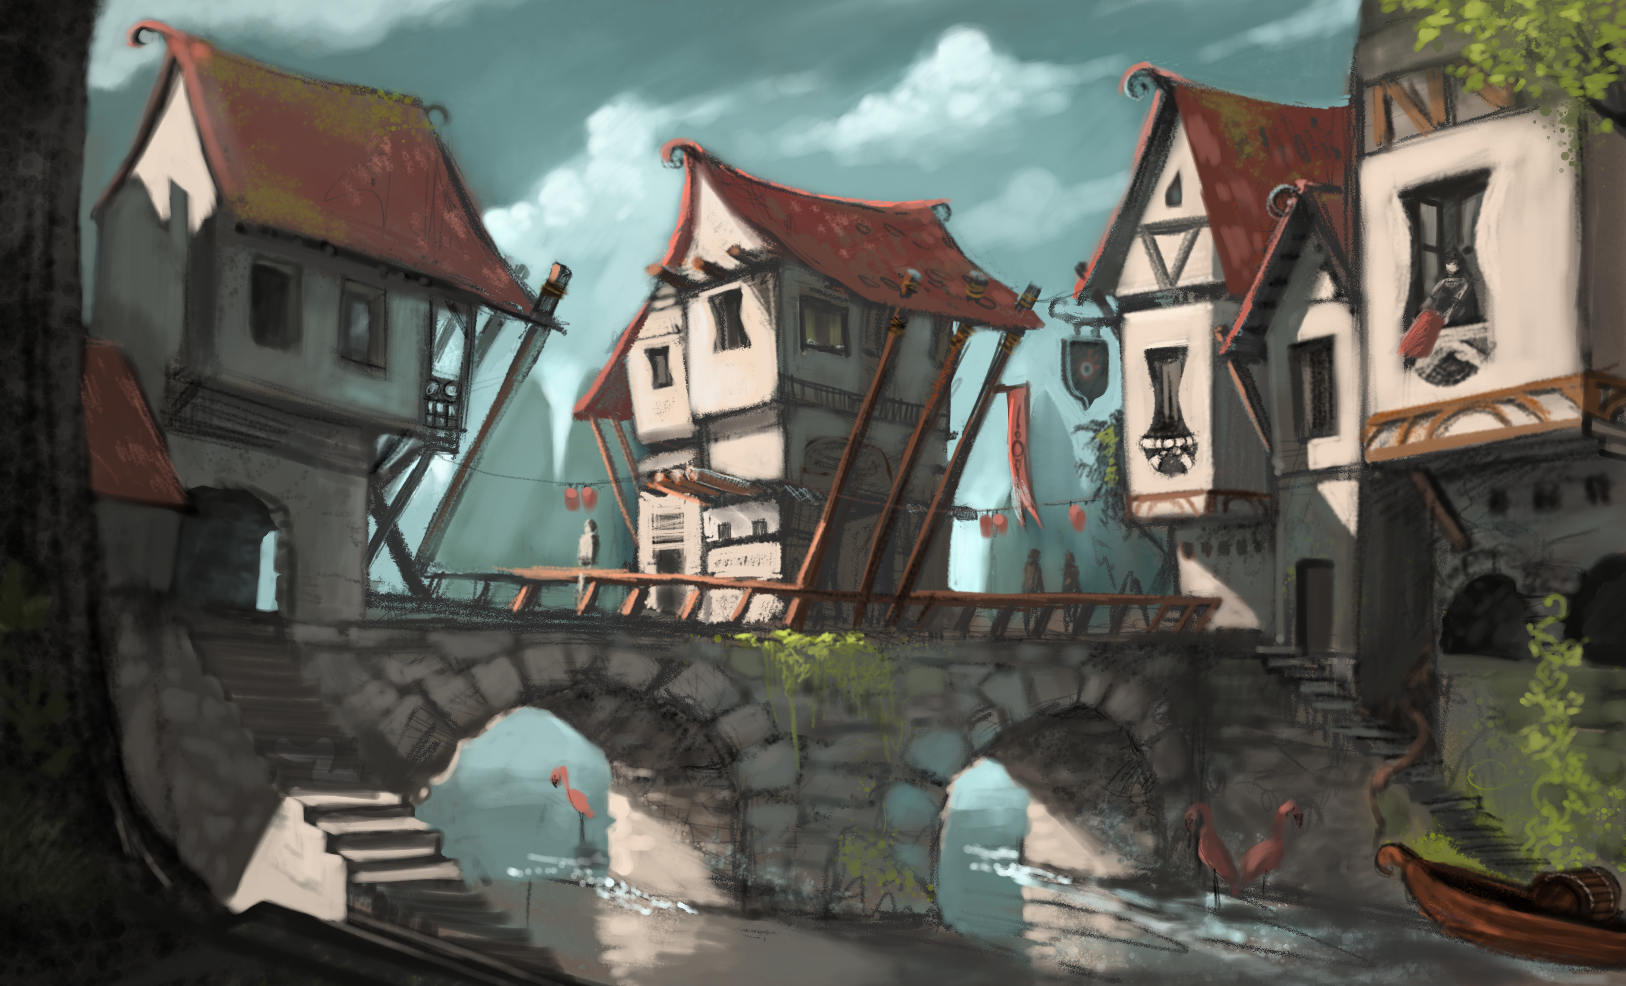
\includegraphics[width=0.80\textwidth]{bridge.png}
    \hfill
  \caption {\tiny By David Revoy / Blender Foundation - Own work, CC BY 3.0}
\end{figure*}
    Tales of Kornwal est un jeu vidéo basé sur les mêmes règles de Fallout Tactics, \textit{i.e}  un jeu d'aventure doté d'un système de combat en tour par tour, permettant aux joueur de progresser et interagir avec un univers à l'allure originale à mi-chemin entre le médiéval-fantastique et le post-apocalyptique.
    
    Les interactions seront basées sur un système de gestion d'inventaire et d'au moins une caractéristique, qui feront office de modificateurs lors d'actions enterprises par le personnage (\textit{e.g} : la caractéristique "Force" influera grandement sur les dégâts infligés par un ennemi ou par le héros, ainsi que l'utilisation de telle ou telle arme).
    
    \section{Règles du jeu}
    Le jeu pourra posséder plusieurs aspects dépendant de l'étude du cahier des charges :
    \par\leavevmode\
\begin{itemize}
\item Déplacement d'un personnage sur une "zone" de la mappemonde, accédant aux différentes cases nord-sud-est-ouest de la map en cliquant sur l'une des extrémités de l'écran.
\par\leavevmode\

\item Système de combat tour par tour : lors d'une rencontre avec un ennemi, la map se vide de tous les sprites autres que le personnage joueur et ses adversaires, laissant donc place au duel entre le héros et l'ennemi. Le joueur commencera en premier (sauf modification) et disposera de deux choix possibles : se déplacer d'une case dans la zone, ou attaquer l'ennemi, faisant baisser son capital de points de vie. Le nombre de points de vie retirés dépendra de la caractéristique FORCE du personnage, ainsi que de son ARME équipée. Le tour se termine après que l'une des actions suivante a été effectuée, laissant le tour à l'ennemi (qui se déroulera de la même manière).






\par\leavevmode\

\item Système d'interaction avec les personnages joueur ou non-joueur (discussions, interface d'échange d'objets)
\end{itemize}

    \chapter{Description et conception des états du jeu}
    
    \section{Description des états}
    Un état du jeu est défini par les éléments suivants :
    
\begin{itemize}
    

    \item  \textbf{Les élements d'espace} (classe Space), élément immobiles permettant de définir les zones où les personnages peuvent se déplacer (\textit{e.g} herbe, sable, neige...). Sur les bords de la zone (définie par la grille, constituée des éléments fixes Space et Wall), l'attribut booléen "changemap" est "True", ce qui permet au personnage de changer de zone.
   \par\leavevmode\

    \item  \textbf{Les élements de mur} (classe Wall), définissant les zones où un personnage ne peut se déplacer (\textit{e.g}  mur)
    
         
\par\leavevmode\
    \item \textbf{Les personnages} (classe Character), éléments mobiles se déplaçant sur la grille (ou plus exactement sur les cases définies par les classes Space). Ces éléments peuvent être contrôlés soit par l'humain (Personnage joueur), soit par les IA (Personnages non joueurs). Les personnages possèdent trois status possibles :
    \begin{itemize}
    
    \item YOURTURN : Le tour du personnage. Il aura le droit de dépenser des points de mouvements pour se déplacer sur la map, ou des points d'actions pour endommager les adversaires.
    \item HISTURN : Le tour des autres personnages. Le personnage doit rester immobile et subir les actions des autres personnages jusqu'à ce que son tour arrive.
    \item  DEAD : Le personnage ne peut plus bouger, son tour n'arrivant jamais. Il est mort.
    \end{itemize}
    
    \end{itemize}
    
    	\section{Livrable, Jalon 1}
    
	\section{Livrable, Jalon 1}
    
    \chapter{Changelog}
    \section{Livrable, Jalon 1}
    \begin{itemize}
\item \textbf{Date}  : Mercredi 28 Septembre 2016

\par\leavevmode\
\item \textbf{Version}  : 1.1

\par\leavevmode\
\item \textbf{Nature de l'ajout sur le rapport}  : \begin{itemize}\item Ajout des textures et des effets sonores \item Page de garde \item Sommaire \item Section 1.1 : Présentation générale \item Section 2.2 : Règle du jeu \end{itemize}

\par\leavevmode\
\item \textbf{Modifications}  : Aucune modification pour l'instant.\end{itemize}
    
    
\end{document}
